\documentclass[a4paper,11pt,twocolumn,twoside]{article}
\usepackage[dvips]{graphicx}
\usepackage{sepln}
\usepackage{fullname_esp}
\usepackage[utf8]{inputenc}
\usepackage[spanish,es-nosectiondot, es-tabla, es-noindentfirst, es-nolists]{babel}

\input epsf



\setlength\titlebox{4in} %esto por defecto

\title{Extracción automática de argumentos en textos de opinión en la prensa cubana}

\author {\textbf{Luis Ernesto Ibarra Vázquez,$^1$} \textbf{Damian Valdés Santiago$^1$}\\
$^1$Universidad de la Habana\\
% $^2$Universidad de la Habana\\
luise98cu@gmail.com, damian@correo.com\\ % TODO poner el correo de Damian
}

\seplntranstitle{Automatic argument extraction in opinion texts in cuban press}

\seplnclave{Extracción de argumentos, } % TODO Seguir en esto

\seplnresumen{El estudio de la argumentación en la prensa cubana es un campo en donde se han reportado
relativamente pocas investigaciones. En estos estudios es posible obtener 
información de los esquemas argumentativos utilizados en los textos y
realizar acciones en base a estos.
Este problema tradicionalmente es resuelto mediante 
una anotación manual por expertos en lingüística, trabajo que se 
caracteriza por tomar mucho tiempo y recursos. La Extracción
de Argumentos es la rama del Procesamiento del Lenguaje Natural
encargada de estudiar algoritmos y métodos para solucionar los problemas
asociados a la anotación de las estructuras argumentativas. Mediante el uso 
de estos es posible automatizar el procedimiento de anotación
de la argumentación. 
En este trabajo se propone la anotación de textos argumentativos
mediante el uso de dos modelos de aprendizaje profundo, entrenados con 
conjuntos de datos traducidos y proyectados del inglés, encargados de resolver
las tareas relacionadas al problema. 
El primer modelo propuesto 
consiste en uno secuencia a secuencia usado para la extracción y clasificación
de las unidades de discurso argumentativas (UDA) mediante el uso de \textit{Long Short Term Memory} 
(LSTM) y \textit{Conditional Random Field} (CRF). Para la extracción y clasificación de 
enlaces entre las UDAs se propone un modelo de clasificación basado en redes residuales,
atención y LSTM. Ambos modelos utilizan \textit{embeddings} GloVe para la representación 
de las palabras. Los resultados obtenidos en la extracción de UDAs alcanzaron valores de
0,82 en la métrica F1 comparados con 0,85 obtenidos en el estado del arte. 
En las demás tareas, los resultados no son directamente comparables con los del estado del arte, 
los mejores valores F1 obtenidos fueron 0,56 en la clasificación de UDAs, 0,74 en la predicción
de enlaces y 0,39 en la clasificación de enlaces.
Con dichos modelos se anotaron las ``Cartas a la Dirección'', del 
periódico Granma, creándose un conjunto de datos con las estructuras argumentativas anotadas
y listas para el estudio de estas por lingüistas.}


\seplnkey{Argument extraction, } % TODO Seguir en esto

\seplnabstract{The study of argumentation in the Cuban press is a field in which relatively little
research has been reported. In these studies it is possible to obtain information on 
the argumentative schemes used in the texts and take actions based on them. This problem
is traditionally solved through manual annotation by linguistic experts, a work that takes 
a lot of time and resources. Argument Extraction is the branch of Natural Language Processing 
in charge of studying algorithms and methods to solve the problems associated with the annotation 
of argument structures. By using these algorithms it is possible to automate the argumentation 
annotation procedure.  In this paper we propose the annotation of argumentative texts by using 
two deep learning models, trained with translated and projected English datasets, in charge of 
solving the tasks related to the problem.  The first proposed model consists of a sequence to 
sequence one used for the extraction and classification of argumentative discourse units (ADUs) 
by using Long Short Term Memory (LSTM) and Conditional Random Field (CRF). A classification model 
based on residual networks, attention and LSTM is proposed for the extraction and classification of 
links between ADUs. Both models use GloVe for word representation. The results obtained in the 
extraction of ADUs reached values of 0.82 in the F1 metric compared to 0.85 obtained in the state 
of the art.  In the other tasks, the results are not directly comparable with those of the state of 
the art, the best F1 values obtained were 0.56 in UDAs classification, 0.74 in link prediction and 
0.39 in link classification. With these models, the ``Letters to the Management'' of the Granma 
newspaper were annotated, creating a data set with the argumentative structures annotated and 
ready to be studied by linguists. }

\firstpageno{1}


\begin{document}

% la siguiente instrucción sólo se debe usar si el abstract sobrescribe el texto
% la longitud variará según se necesite

%\setlength\titlebox{20cm} % se aumenta el tamaño del espacio reservado para datos de título


\label{firstpage} \maketitle

%\begin{abstract}
%Resumen del artículo con una sangría a izquierda y derecha de 0.32
%cm, justificado por ambos lados, con tamaño de fuente 11.
%
%\end{abstract}

\section{Instroducción}

La argumentación es una actividad verbal, social y racional destinada a convencer 
a un crítico razonable de la aceptabilidad de un punto de vista mediante la presentación 
de una constelación de proposiciones que justifican o refutan la proposición expresada 
en el punto de vista [\cite{van2004systematic}]. Esta definición concentra en ella 
partes esenciales de lo que es la argumentación, dicha actividad se encuentra presente
en varias facetas de la cotidianedad humana, como en la escritura o lectura de documentos y
en las interacciones sociales de las personas. En resumen, la argumentación está presente 
cada vez que se plantea un argumento y se trata de que este triunfe en un debate donde 
se exponen elementos que lo apoyen.   

En la actualidad es necesario tener acceso a la información
de forma rápida y simple. Esto no siempre es posible dado la gran cantidad de información existente y
que es generada en cada momento. En caso de tener una vía de acceder a esta, se podrían realizar acciones
con mayor rapidez y calidad. Con la argumentación, se podría hacer explícitas las razones de las personas 
al afirmar algo sobre un tema teniendo así su punto de vista individual, y con suficientes personas, colectivo.

% Antecedentes del problema, justificación y motivación. 
% Antecedentes: 
%   Tareas similares que se quedan cortas: Opinion Mining, Citation Mining, Controversy Detection
%   Cómo se ha estudiado primero a mano. Trabajo dificil.
% Justificacion:
%   Limitaciones del trabajo manual
%   Se quiere hacer el trabajo automatico.
%   El proyecto esta integrado en un proyecto nacional  reconocido CORESPUC

Varias tareas en el Procesamiento de Lenguaje Natural (PLN) se han desarrollado en 
torno a diferentes problemas relacionados con 
la argumentación. Entre tales tareas se encuentran: el minado de opiniones, el cual es el 
estudio computacional de las opiniones, sentimientos y emociones expresadas en un texto 
[\cite{liu2010sentiment}], la detección de controversias, enfocada en la identificación de 
temas y textos en donde puntos de vista conflictivos están presentes; y también la zonificación
argumentativa que clasifica las oraciones por su rol argumentativo dentro de un artículo
científico. Estas tareas solamente muestran cuáles opiniones, puntos de conflictos y roles 
de argumentos 
presenta el texto, pero lo realizan de manera separada y no muestran el porqué de estas. 
Para lograr extraer esta información faltante es necesario realizar un 
análisis de los argumentos dados, para pasar de texto no estructurado a datos argumentativos 
que den entendimiento de los puntos de vista y de cómo se apoyan o atacan entre sí. Este análisis
es posible realizarlo mediante métodos convencionales manuales o utilizando programas
especializados para la anotación, aunque la práctica ha demostrado que este proceso requiere 
de una gran cantidad de tiempo y de personal calificado. Con la inmensa cantidad de datos 
que se genera a diario este análisis es impracticable de realizar de forma manual, por esto se 
estudian y crean métodos encargados de automatizar esta tarea.

% Breve presentación de la problemática. 
%   Por todo lo anterior nace la EA, rama de PLN ..., definir tareas de la EA, tocar los enfoques realizados
% (No es el estado del arte aunque se puede hablar un poco de él) Elementos involucrados en el punto de vista cientifico, lleva corpus.

La Extracción de Argumentos (EA) nace como la rama del PLN encargada
del estudio de métodos para la extracción automática de las estructuras argumentativas de 
los textos y su posterior procesamiento [\cite{lawrence2020argument}]. Esta tarea se divide en 
cuatro subtareas fundamentales: i) la extracción y ii) clasificación de las componentes 
argumentativas del texto, y iii) la extracción y 
iv) clasificación de las relaciones entre estas. Estas tareas han sido abordadas de diferentes maneras,
desde modelos secuenciales [\cite{palau2009argumentation}, \cite{goudas2015argument}] hasta 
\textit{end-to-end} [\cite{eger2017neural}], desde el uso de clasificadores clásicos 
como Naive Bayes o SVM [\cite{niculae2017argument}, \cite{stab2017parsing}] hasta el uso de 
aprendizaje profundo [\cite{galassi2021deep}, \cite{mayer2020transformer}], y sigue 
siendo un área creciente de estudio.

La EA se caracteriza por la falta de conjuntos de datos y 
por la heterogeneidad que presentan estos a la hora de decidir cómo realizar las 
anotaciones, además que la gran mayoría de los estudios realizados en el campo se encuentran en 
un reducido conjunto de idiomas como el inglés, alemán o chino [\cite{eger2018cross}]. 
En el español, pocas intervenciones se han dado en el análisis de los argumentos [\cite{esteve2020mineria}] y en 
lo correspondiente a Cuba no se encontró ninguna referencia. 

% Diseño teórico.
%    Problema: 
%    Objeto de Investigación: Procesamiento de Lenguaje Natural
%    Campo de acción: Linguistica computacional
%    Hipótesis o preguntas científicas
%    Objetivos generales y específicos
%       General: Diseño e implementación de un algoritmo para el estudio de la argumentación en el periódico digital Granma
%       Especifico Construcción del corpus de los periódicos: Crawler, Anotación (scpaCy).
%       Especifico Implementacion de la interfaz gráfica para consultar los resultados.

En esta tesis se tiene como objetivo, proponer un algoritmo para 
la extracción y análisis de estructuras argumentativas en textos 
de la prensa cubana, constituyendo el primero de su tipo en lo que respecta a la búsqueda del autor. 
Para lograr dicho objetivo se necesitan realizar varias operaciones.
En primer lugar, es necesario obtener los textos a analizar del sitio 
web del periódico Granma. Luego, se necesita confeccionar algoritmos capaces de realizar las tareas 
de EA sobre estos textos, para estos algoritmos es necesaria la confección de conjuntos 
de datos en español en los cuales se puedan entrenar. Finalmente, se requiere de una interfaz visual 
en la que sea posible la interacción de los usuarios, en tareas como visualización y edición, 
con los resultados obtenidos. 

Se propone la construcción de un programa capaz de realizar la extracción de los textos del periódico Granma, 
en específico, se enfoca en su sección de Cartas a la Dirección. Para la extracción
de argumentos se presentan dos modelos, el primero se encarga de la segmentación y clasificación
de las componentes argumentativas. Este es un modelo secuencia a secuencia en el cual las palabras 
son vectorizadas por sus características morfológicas mediante el uso de redes neuronales convolucionales
(CNN) y \textit{Long Short Term Memory} (LSTM), por su información
semántica mediante \textit{embeddings} \textit{Global Vectors} (GloVe) y por su información 
estructural mediante su parte de la oración, estas 
secuencias son procesadas por una red LSTM bidireccional y sus atributos son usados por una capa 
de \textit{Conditional Random Field} (CRF) 
para su clasificación final en etiquetas B (inicio de segmento), I (dentro del segmento), O (afuera de segmento), 
E (fin de segmento) y S (segmento de un elemento) (BIOES) con información adicional para la clasificación de las 
unidades de discurso argumentativas (UDA). El segundo modelo está encargado de la extracción y clasificación 
de las relaciones entre las UDAs. En él se utilizan las representaciones GloVe de las palabras en las secuencias 
y su distancia argumentativa para la clasificación de una tupla en la que su primer elemento 
constituye el texto candidato de donde parte la relación o fuente y el segundo, el texto candidato a recibir la 
relación u objetivo, en el tipo de relación existente entre estos elementos. La entrada es procesada mediante 
una LSTM bidireccional y módulos de atención cruzada entre los elementos de la fuente y los elementos del objetivo.
Para la visualización se crea un ambiente de desarrollo con la herramienta Brat [\cite{brat}], la cual permite realizar las 
tareas requeridas a los datos anotados por los modelos.

En resumen, se presenta un estudio de la argumentación en español al realizar la extracción de 
argumentos en prensa, además se crea un conjunto de datos anotado que puede servir
para un estudio más profundo sobre los esquemas argumentativos presentes en estos textos. 

\section{Marco teórico}


\section{Argumentación}

La argumentación es un tema tratado desde la antigüedad, Aristóteles lo defendía como la 
habilidad de, dada una pregunta, considerar los elementos útiles para persuadir a alguien, algo
similar a la retórica. De una perspectiva más contemporánea surgen las ideas de 
\textcite{perelman1969rhetoric}
enfocadas en un análisis de la retórica en donde se estipula que la teoría de la argumentación
responde a provocar o aumentar la adhesión de las personas a las tesis presentadas, por medio de 
técnicas discursivas. En 
\textcite{toulmin_2003}
se considera como argumento todo aquello que ofrece, 
o todo lo que es utilizado, para justificar o refutar una proposición. En este último, se toma 
una perspectiva más racional y deductiva de la argumentación, dando como resultado lo que se 
conoce como el Método de Toulmin. 

\subsection{Método de Toulmin}

Este método divide los argumentos en seis partes: afirmación 
(\textit{claim}), fundamento (\textit{grounds}), justificación (\textit{warrant}), calificador 
(\textit{qualifier}), refutación (\textit{rebuttal}) y respaldo (\textit{backing}).
Mediante las afirmaciones se conoce el argumento principal que el autor quiere probar a la audiencia,
estas son respaldadas con fundamentos, siendo estos las evidencias y hechos en que se apoya el autor.
Las justificaciones pueden estar explícitas o implícitas y son suposiciones que vinculan los
fundamentos con las afirmaciones, estas a su vez pueden ser respaldadas por conocimiento.
El esquema introduce la posibilidad de otra situación válida a la establecida en las afirmaciones
mediante la refutación. Los calificadores son usados para dar más información de la calidad o seguridad
de las afirmaciones dadas. Un ejemplo\footnote{Extraído de  
\textcite{toulminArgument}.
} de este esquema es:

\begin{adjustwidth}{25pt}{25pt}
    [\textit{Se escucharon ladridos y aullidos en la distancia}]$_{\mathrm{fundamento}}$, 
    [\textit{probablemente}]$_{\mathrm{calificador}}$ 
    [\textit{haya perros en las cercanías}]$_{\mathrm{afirmación}}$.
\end{adjustwidth}

En este ejemplo, además de las partes explícitas, se encuentran partes implícitas como la justificación 
(\textit{los perros son animales que ladran y aúllan}), el respaldo (\textit{se sabe que existen perros en la zona}) y 
la refutación (\textit{puede ser que hayan lobos o coyotes cerca}).

Este método crea una definición compacta que ayuda a los investigadores a enfocar su búsqueda 
en las diferentes categorías definidas. Además, engloba de manera comprensible un tema tan complejo 
como la argumentación al tomar en cuenta gran parte de los elementos presentes en el razonamiento
realizado para llegar a conclusiones, incorporando incluso elementos probabilísticos en el proceso. 

\subsection{Rasgos lingüísticos}

Los rasgos lingüísticos son aquellas características que se encuentran presentes en los textos 
que hacen que estos se clasifiquen argumentativos [\cite{venegas2005hacia}]. Con 
la identificación de estos se hace la tarea de extracción más sencilla y con un marco teórico 
que respalde las decisiones tomadas. Ejemplos de rasgos presentes en textos argumentativos:

\begin{enumerate}
    \item Marcas de orden que introducen párrafos: \textit{primero}, \textit{segundo}, \textit{por un lado}, 
    \textit{por otra parte}, \textit{finalmente}.
    \item Comillas y citas: citar palabras que refuercen la intervención recurriendo a autoridades
    o personajes.
    \item Nexos que expresan causa o consecuencias: \textit{ya que}, \textit{porque}, \textit{pues}, 
    \textit{con motivo de}, \textit{gracias a}, \textit{considerando que}, \textit{por lo tanto}, \textit{de manera que}.
\end{enumerate}

Estos rasgos además de dar indicación de la existencia de argumentos dan pie para conocer las relaciones
entre estos y los tipos de argumentos. Por ejemplo, \textit{por lo tanto}, implica que lo que viene 
a continuación es una conclusión apoyada en lo dicho anteriormente en el texto. Algo parecido
sucede con \textit{ya que}, en este caso implica que lo siguiente es un argumento que se encuentra 
relacionado con lo mencionado antes.

En
\textcite{venegas2005hacia}
se determinan 16 categorías y 51 rasgos lingüísticos, dando una idea 
de la gran variedad de marcadores presentes en la argumentación.

\section{Extracción de Argumentos}

El PLN es un subcampo de la Inteligencia Artificial que tiene como objetivo la comprensión 
del lenguaje humano por las computadoras. 
Mediante el uso de sus algoritmos es posible el procesamiento masivo de texto para la extracción de información 
relevante de este. Entre las tareas pertenecientes a dicho campo se encuentran la Traducción Automática, 
la Generación de Lenguaje Natural y la Extracción de Argumentos (EA). La EA constituye la identificación y extracción 
automática de las estructuras de inferencia y 
razonamiento expresadas como argumentos presentes en el lenguaje natural [\cite{lawrence2020argument}].
En la actualidad, tareas del PLN como el análisis de sentimientos permiten 
extraer cuáles son las opiniones o sentimientos presentes, sin embargo, este análisis presenta una falta 
de información, ya que no justifica el porqué de las opiniones. La EA permite dar respuesta a este problema presentando
los argumentos y cómo sus relaciones justifican las posiciones del hablante. Dicho problema está constituido por diferentes 
estructuras y se compone de distintas tareas necesarias para su solución.

\subsection{Estructuras Argumentativas}

Las estructuras argumentativas son las partes de la argumentación de los textos y sus relaciones.
Estas se componen de dos elementos principales: las Unidades de Discurso Argumentativas (UDA) y los enlaces
existentes entre estas. Las UDAs corresponden a la unidad mínima de argumentación, definida 
como un segmento de texto que juega un solo rol para el argumento analizado, y es 
delimitado por segmentos vecinos que tienen roles diferentes o ningún rol [\cite{stede2018argumentation}].
Las UDAs se relacionan entre sí conformando el proceso de inferencia y razonamiento del argumento.
Tanto los enlaces como las UDAs son clasificados en dependencia de su rol en la argumentación, estas clasificaciones 
en las UDAs parten de los conceptos de afirmación, declaración controversial y parte central del argumento, y premisa,
razones que la justifican o refutan, y en las relaciones de ataque y apoyo. 

\subsection{Tareas de extracción de argumentos}

Dada la definición de estructuras argumentativas y que el objetivo de la EA es extraerlas,
se conciben las siguientes tareas principales:

\subsubsection{Extracción de UDAs}

Consiste en la separación de los segmentos de texto que formarán parte de la estructura.
En este proceso el texto es segmentado y se obtiene un conjunto de UDAs. En el siguiente 
ejemplo\footnote{Traducido del corpus de 
\textcite{stab2017parsing}
.} se representa 
la extracción de UDAs marcadas en \textit{cursiva} de un texto dado:

\begin{adjustwidth}{25pt}{25pt}
    En primer lugar, [\textit{el correo electrónico puede contar como uno de los resultados
    más beneficiosos de la tecnología moderna}]. [\textit{Años atrás, las personas pagaban gran cantidad de dinero para 
    enviar sus cartas y sus pagos estaban sujetos al peso de sus cartas o paquetes y muchos accidentes podrían 
    causar problemas que causarían que el correo no fuera enviado}].
\end{adjustwidth}

\subsubsection{Clasificación de UDAs}

La clasificación de UDAs consiste en asignarle la categoría que toma la UDA en la argumentación. En general, 
las clasificaciones parten de dos clases bases, las afirmaciones y premisas, aunque estas pueden ser tantas
como sea necesario por el problema específico a tratar. Siguiendo con el ejemplo, se observa la clasificación
en afirmación y premisa asignada a los segmentos extraídos en el paso anterior:

\begin{adjustwidth}{25pt}{25pt}
    En primer lugar, [\textit{el correo electrónico puede contar como uno de los resultados
    más beneficiosos de la tecnología moderna}]$_{\mathrm{Afirmación}}$. [\textit{Años atrás, las personas pagaban gran cantidad de dinero para 
    enviar sus cartas y sus pagos estaban sujetos al peso de sus cartas o paquetes y muchos accidentes podrían 
    causar problemas que causarían que el correo no fuera enviado}]$_{\mathrm{Premisa}}$.
\end{adjustwidth}

\subsubsection{Extracción de relaciones entre las UDAs}

La extracción de relaciones constituye el paso donde se determina si están relacionadas las UDAs o no. 
La disposición de estas relaciones forma el proceso de razonamiento en que se basa el autor para validar 
su posición. En el ejemplo se representa la existencia de relación mediante su distancia argumentativa con 
la UDA con la que se relaciona. La distancia argumentativa es la cantidad de UDAs del texto que separan la 
UDA fuente del objetivo [\cite{galassi2021deep}], en caso de ser negativa (positiva) el objetivo se encuentra 
antes (después) que la fuente.

\begin{adjustwidth}{25pt}{25pt}
    En primer lugar, [\textit{el correo electrónico puede contar como uno de los resultados
    más beneficiosos de la tecnología moderna}]$_{\mathrm{Afirmación}}$. [\textit{Años atrás, las personas pagaban gran cantidad de dinero para 
    enviar sus cartas y sus pagos estaban sujetos al peso de sus cartas o paquetes y muchos accidentes podrían 
    causar problemas que causarían que el correo no fuera enviado}]$_{\mathrm{Premisa, -1}}$.
\end{adjustwidth}

\subsubsection{Clasificación de relaciones entre las UDAs}

La clasificación de las relaciones consiste en clasificar las relaciones extraídas en las categorías pertinentes.
Los tipos de relaciones, nacen de dos clases bases por lo general, las relaciones de apoyo y de ataque.
Las de apoyo son aquellas en las que la UDA fuente afirme la UDA objetivo, las de ataque son 
las que la UDA fuente apoya la negación de la UDA objetivo.

\begin{adjustwidth}{25pt}{25pt}
    En primer lugar, [\textit{el correo electrónico puede contar como uno de los resultados
    más beneficiosos de la tecnología moderna}]$_{\mathrm{Afirmación}}$. [\textit{Años atrás, las personas pagaban gran cantidad de dinero para 
    enviar sus cartas y sus pagos estaban sujetos al peso de sus cartas o paquetes y muchos accidentes podrían 
    causar problemas que causarían que el correo no fuera enviado}]$_{\mathrm{Premisa, -1, apoyo}}$.
\end{adjustwidth}

Partiendo de esto, se puede observar que las estructuras argumentativas de un texto constituyen un grafo dirigido 
en donde sus nodos representan las UDAs y están anotados con su tipo, y sus vértices representan las 
relaciones entre las UDAs. Dichos vértices se anotan con el tipo de relación existente entra ambas 
(Figura \ref{fig:arg_struct}).

\begin{figure}[h]
    \centering
    \includesvg[scale=.7]{Graphics/Estructuras_argumentativas.svg}
    \caption{Estructuras Argumentativas.}
    \label{fig:arg_struct}
\end{figure}

\section{Segmentación y clasificación de UDAs}

Esta primera parte se modela como un problema secuencia a secuencia cuyo objetivo es asignar a los tokens 
extraídos del documento entrada una etiqueta BIOES para segmentar las UDAs. Para la clasificación del tipo 
de UDA, al conjunto de etiquetas BIES se le añadieron las clasificaciones que presenta el corpus entrenante.
En el siguiente ejemplo se muestra una salida del modelo presentando las clasificaciones de
$A$ como argumento y $P$ como premisa:

\begin{adjustwidth}{25pt}{25pt}
    En$_O$ primer$_O$ lugar$_O$ ,$_O$ [\textit{el$_{B-A}$ correo$_{I-A}$ electrónico$_{I-A}$ puede$_{I-A}$ 
    contar$_{I-A}$ como$_{I-A}$ uno$_{I-A}$ de$_{I-A}$ los$_{I-A}$ resultados$_{I-A}$
    más$_{I-A}$ beneficiosos$_{I-A}$ de$_{I-A}$ la$_{I-A}$ tecnología$_{I-A}$ moderna$_{E-A}$}] .$_{O}$ 
    [\textit{Años$_{B-P}$ atrás$_{I-P}$ ,$_{I-P}$ las$_{I-P}$ personas$_{I-P}$ pagaban$_{I-P}$ gran$_{I-P}$ cantidad$_{I-P}$ 
    de$_{I-P}$ dinero$_{I-P}$ para$_{I-P}$ enviar$_{I-P}$ sus$_{I-P}$ cartas$_{I-P}$ y$_{I-P}$ sus$_{I-P}$ 
    pagos$_{I-P}$ estaban$_{I-P}$ sujetos$_{I-P}$ al$_{I-P}$ peso$_{I-P}$ de$_{I-P}$ sus$_{I-P}$ 
    cartas$_{I-P}$ o$_{I-P}$ paquetes$_{I-P}$ y$_{I-P}$ muchos$_{I-P}$ accidentes$_{I-P}$ podrían$_{I-P}$
    causar$_{I-P}$ problemas$_{I-P}$ que$_{I-P}$ causarían$_{I-P}$ que$_{I-P}$ el$_{I-P}$ correo$_{I-P}$ 
    no$_{I-P}$ fuera$_{I-P}$ enviado$_{E-P}$}] .$_{O}$
\end{adjustwidth}

\subsection{Modelo de segmentación y clasificación de UDAs}

Sea $D$ un documento entrada, este es separado en una secuencia de $n$ tokens $D_i$ donde $n$ es la mayor longitud encontrada
en los documentos del conjunto de datos (si la cantidad de tokens es menor que $n$ entonces $D_i$ es completado con un token especial de enmascarado). 
A cada token se le asigna
su representación vectorial GloVe de dimensión $g=300$, dando como resultado $G_{ij} \in \mathbb{R}^{n \times g}$.
Esta representación inicial presenta información semántica de las palabras y conserva las relaciones 
espaciales entre ellas. 

Para la representación de información morfológica de la palabra se construyen dos
codificadores que procesan los caracteres de cada token y devuelven una representación vectorial de estos.
A cada caracter se le asigna un vector que será entrenado convirtiendo un token en un vector de dimensión
$q \times c$, donde $q$ es el tamaño máximo de palabra en el conjunto de datos y $c$ es la dimensión del vector
asignado a cada caracter.
Uno de estos modelos está basado en CNN, este modelo entrena una representación de caracteres de dimensión
$cd=50$ representando un token como un vector de dimensión $q \times cd$. Se conforma por una capa de convolución unidimensional
con $f=30$ filtros y un kernel de tamaño $k=3$, seguida por una capa \textit{max pooling} que convierte la secuencia en un vector
de dimensión $1 \times f$, que luego es concatenado a la representación del token a que pertenece.
Otro modelo utilizado para calcular una representación morfológica se encuentra basado en RNN. Se usó
un modelo LSTM bidireccional con dimensión $l=25$ para calcular la representación del token, para las dimensiones de los caracteres se
utilizan vectores de tamaño $l$, el resultado final constituye la concatenación de la corrida hacia adelante y
hacia atrás formando una representación de dimensión $1 \times 2 \cdot l$ del token. Este vector es concatenado a la representación
del token correspondiente. Otro atributo usado en la representación de los tokens constituyen las etiquetas de 
Partes de la Oración de estos.
El conjunto de etiquetas elegido es un conjunto universal [\cite{petrov2011universal}] aplicable a cualquier idioma.
De estas etiquetas se les extrae la codificación \textit{one-hot} y esta es transformada por una capa densa con $p=5$ neuronas
y función de activación \textit{ReLU}, el resultado es concatenado a la representación del token correspondiente. Mediante 
la extracción de estos atributos el token es representado en tres maneras, semántica, morfológica y estructural, con el 
objetivo de que sean aprendidas los rasgos lingüísticos correspondientes a la tarea.

Del proceso de vectorización sale un vector con dimensión $n \times t$ donde $t$ es la dimensión final de la representación
de los tokens. Este vector es modificado por una capa LSTM bidireccional de dimensión $m=200$, a esta salida se le 
añade una conexión residual al ajustarle la dimensión con una capa densa. Luego, la secuencia es procesada por una 
capa densa de dimensión $k=100$ con activación \textit{ReLU} produciendo una representación final de dimensión 
$n \times k$. Finalmente, se utiliza una capa CRF
para la clasificación final de la secuencia en las etiquetas finales. El resultado final constituye un vector
de dimensión $n$ que representa las clasificaciones inferidas por el modelo (Figura \ref{fig:segmenter_model}).

Para prevenir el sobreajuste se agregaron capas de normalización y de \textit{dropout} entre cada proceso y se usaron regularizaciones
L2 y \textit{dropout} en las capas densas y LSTM, el valor asignado al dropout es de $0.5$. 
Para prevenir el sobreentrenamiento se aplicó una 
terminación temprana de este cuando no se encontraba una mejora de la función de pérdida en el conjunto de validación
por más de 10 épocas consecutivas. Como optimizador se utilizó Adam con una tasa de aprendizaje de $0.001$.

\subsection{Posprocesamiento de segmentación y clasificación de UDAs}

La salida del modelo constituye una secuencia de etiquetas en formato BIOES. Esta está propensa
a contener errores en su formato, por ejemplo, secuencias no terminadas en E, segmentos continuos con más de una 
meta-etiqueta, entre otros.
Para la corrección de la estructura se propone el siguiente algoritmo con dos partes. La primera
consiste en arreglar la estructura BIOES, para esto se mantiene una ventana de tamaño
3, [\_ , \_ , \_], sobre la secuencia y se asume que la parte anterior a la posición de la ventana no presenta errores. Al encontrar una
ventana inválida se necesita observar la siguiente ventana para poder decidir cómo se arregla el error, ya que se
podría dar el caso que se observe [O, O, I] y la próxima sea [O, I, O], en donde solamente viendo la primera ventana no se podría saber si el cambio 
correcto corresponde a sustituir I por B o por S. Una vez observadas las dos ventanas, se procede a realizar el 
arreglo correspondiente. En casos donde sea ambigua la manera de arreglar la ventana, [I, I, O] por ejemplo
(La I o la O pueden ser 
sustituidas por una E), se utiliza una función que recibe un segmento y devuelve la gravedad del error.
El error con mayor gravedad será arreglado, en caso de ser iguales se arreglará la etiqueta más a la izquierda.
Este procedimiento devuelve una secuencia BIOES correctamente anotada, debido a que a partir de una secuencia sin 
errores en cada paso se va arreglando la ventana y una vez esta llega al final arregló todos los elementos de la secuencia.
Una vez la secuencia tiene la estructura BIOES correctamente anotada el problema
consiste en arreglar las meta-etiquetas, ya que una misma secuencia BIOES pudo haber sido anotada con diferentes
tipos, en este caso se toma la etiqueta más representativa del segmento continuo.

\begin{figure}[h]
    \centering
    \includesvg[scale=.65]{Graphics/Modelo_Segmenter_UDA.svg}
    \caption{Segmentador UDAs.}
    \label{fig:segmenter_model}
\end{figure}

\newpage

\section{Predicción y clasificación de enlaces}

En esta segunda parte el modelo se encarga de las tareas de extracción y clasificación de enlaces.
El problema consiste en clasificar pares de UDAs, representando origen y objetivo del enlace, 
en el tipo de relación que existen entre estas.
Como tarea auxiliar se clasifican los tipos de UDAs que intervienen en la relación. La salida 
del modelo constituye en una tupla de tres elementos: la clasificación de la relación, 
la clasificación de la UDA origen, la clasificación de la UDA objetivo. Si el enlace existe o no 
es calculado partir de la clasificación de la relación.   

\subsection{Modelo de predicción y clasificación de enlaces}

Sean dos UDAs, $S$ y $T$, donde $S$ representa la fuente de la relación, mientras que $T$ representa
al objetivo. Estas secuencias son tokenizadas y se les asigna la representación GloVe de cada palabra, obteniendo
dos vectores de dimensión $u \times g$, donde $u$ es el tamaño máximo de UDAs en el conjunto de entrenamiento
y $g=300$ es la dimensión del \textit{embedding}.
Estos vectores son modificados por una red densa compuesta por $ca = 4$ capas con activación \textit{ReLu}
de dimensiones $50$, $50$, $50$, $300$, añadiendo una conexión residual a la salida de esta. 
El próximo paso consiste en aplicar una capa densa de dimensión $di=50$ y luego un \textit{average pooling}
de tamaño $dp=10$, obteniendo vectores de dimensión $\frac{q}{dp} \times di$. 
Estos vectores son modificados por un LSTM bidireccional con $lm=50$ unidades. Un módulo de atención es aplicado 
sobre los vectores fuentes, 
en este actúan como consultas el promedio de los vectores objetivo y como llaves y valores los vectores fuentes,
el procedimiento simétrico es realizado para los vectores objetivos.
La salida de los procesamientos son concatenados con la distancia argumentativa obteniendo una representación 
conjunta de la relación a analizar. Esta representación conjunta es modificada por una red residual obteniendo
una representación final de dimensión $l=20$ y luego sometida a los clasificadores de relación y de tipos de UDAs
(Figuras \ref{fig:link_predictor_model1} y \ref{fig:link_predictor_model2}).

Para prevenir el sobreajuste se agregaron capas de normalización y de \textit{dropout} entre cada 
proceso y se usaron regularizaciones L2 y \textit{dropout} en las capas densas y LSTM, 
todos los \textit{dropout} tienen valor $dr=0,1$. Para prevenir el sobreentrenamiento se aplicó una 
terminación temprana de este cuando no se encontraba una mejora de la función de pérdida en el 
conjunto de validación durante $v=5$ épocas consecutivas. Como optimizador se utilizó Adam con descenso 
exponencial con tasa de aprendizaje $lr=0.003$.

Dado que se realiza un aprendizaje de varias tareas, se tienen varias funciones de pérdida individuales que conforman 
la función de pérdida final $e$. Sea $e_r$ la función de pérdida de la clasificación de la relación, $e_s$ la del tipo de UDA origen  
y $e_t$ del tipo de UDA objetivo, entonces $e = 10 \cdot e_r + e_s + e_t$.

\subsection{Preprocesamiento de predicción y clasificación de enlaces}

El uso de este modelo se concreta a nivel de documento, en donde ya se tienen las UDAs extraídas. Para alimentar
al modelo con los pares de UDAs y sus distancias argumentativas se seleccionan todos los pares de estos que cumplan
que no se enlacen con ellos mismos, por ejemplo, $a \rightarrow a$; y que su distancia argumentativa absoluta sea menor 
que $da=10$. Estas restricciones disminuyen el número de pares extraídos por documentos a una cantidad lineal 
con respecto a la cantidad de UDAs, presentes ya que por cada UDA solamente se tomarían $2 \cdot da$ elementos como máximo
(los que la preceden y los que la suceden). 

Además de las etiquetas $R$ originales del conjunto de entrenamiento, se añaden elementos extras a este
conjunto. Estos elementos son las representaciones inversas de las relaciones, por ejemplo, si $a \xrightarrow{c} b$ entonces 
se agregará el par $b \xrightarrow{c^{-1}} a$, donde $c^{-1}$ es una nueva clasificación de relación que representa
el inverso de la clasificación $c$. Este proceso se realiza para aumentar la cantidad de relaciones positivas en el
conjunto entrenante, ya que aun con las reducciones hechas existe un desbalance de clases positivas y negativas en
las relaciones.

\subsection{Posprocesamiento de predicción y clasificación de enlaces}

Se calcula una salida extra a partir de las distribuciones de probabilidad de las relaciones 
devueltas por el modelo, esta salida representa si el par está enlazado o no directamente, para este cálculo se 
suman las categorías vinculadas a las clases originales del conjunto de datos, esta se toma como la probabilidad de estar 
enlazados, que en caso de ser mayor del 50\% se devuelve verdadero. Para dar el resultado final se eliminan del 
conjunto de respuesta las relaciones anotadas con las etiquetas inversas añadidas en el paso de preprocesamiento 
y son devueltas aquellas que se clasifiquen como enlazadas según el criterio anterior.

\newpage

\begin{figure}[h]
    \centering
    \includesvg[scale=.6]{Graphics/Modelo_Link_Prediction1.svg}
    \caption{Predictor de enlaces.}
    \label{fig:link_predictor_model1}
\end{figure}
\begin{figure}[h]
    \centering
    \includesvg[scale=.6]{Graphics/Modelo_Link_Prediction2.svg}
    \caption{Predictor de enlaces (continuación).}
    \label{fig:link_predictor_model2}
\end{figure}

\section{Conclusiones}

En el trabajo se logró la extracción de estructuras argumentativas en los textos de las 
Cartas a la Dirección del periódico Granma. Para esto se 
extrajeron los textos de las Cartas creando un conjunto de datos
conteniendo, no solo el texto de las cartas, si no, los comentarios 
escritos por los usuarios e información sobre la carta a la que responde, si es una respuesta.
Se creó un software que puede ser utilizado no solo para el trabajo con las Cartas a la Dirección, si no
que este permite un uso general para las tareas de proyección de corpus y trabajo relacionados a la EA.
Este permite incorporar nuevas componentes haciendo posible una extensión simple y desacoplada. 
Para la anotación de las estructuras se crearon conjuntos de datos en español a partir de conjuntos 
anotados en inglés para poder 
tener datos con los cuales entrenar los modelos propuestos. Estos modelos, uno encargado 
de la segmentación y clasificación de las UDAs, y otro de la extracción y clasificación de las 
relaciones entre estas, fueron utilizados para la anotación de los textos extraídos.
Los resultados obtenidos en la tarea de segmentación se encuentran al nivel del estado del arte,
en las demás tareas no se encontraron comparaciones directas al enfoque tomado en la propuesta,
aunque no teniendo en cuenta esto, se obtienen comparativas inferiores en la clasificación
de UDAs y en la clasificación de relaciones, aunque se supera la métrica de predicción de enlace. 
Los resultados obtenidos del procesamiento de las Cartas a la Dirección son considerados 
aceptables por autor. 


\section{Título de nivel uno}

\subsection{Título de nivel dos}

\subsubsection{Título de nivel tres}

El primer párrafo de la sección no lleva sangría. El resto del
texto vendrá con fuente Times New Roman tamaño 11 y justificado
por ambos lados.

Los siguientes párrafos llevan una sangría en la primera línea de
0,5 cm. El resto del texto vendrá con fuente Times New Roman
tamaño 11 y justificado por ambos lados.


\section{Título de nivel uno}

El primer párrafo de la sección no lleva sangría. El resto del
texto vendrá con fuente Times New Roman tamaño 11 y justificado
por ambos lados\footnote{Ejemplo de nota al pie de página ... Más
texto Más texto Más texto Más texto Más texto Más texto Más texto
Más texto Más texto.}.

Los siguientes párrafos llevan una sangría en la primera línea de
0,5 cm. El resto del texto vendrá con fuente Times New Roman
tamaño 11 y justificado por ambos lados.

\section{Ejemplo de una cita}

Ejemplo de una cita dentro de un párrafo: ``Lo dicho por el
autor...".

Otro ejemplo de cita en un párrafo independiente:

\parbox{6.5cm}{\textit{Texto de la cita, iu poiu poiu poiu poiu poiu poiu poi
upoiu poiu poi upoiu oiu oiupoiu opiu poip.}}

Continuación del texto. El resto del texto vendrá con fuente
Times New Roman tamaño 11 con una sangría en la primera línea de
0,5 cm y justificado por ambos lados.


\section{Ejemplos de tablas y figuras}

Ejemplo de tabla. En la Tabla \ref{tabla1} se muestran los
resultados...
\begin{table} [h]
\begin{center}
\begin{tabular} {|l|c|}
  \hline\rule{-2pt}{15pt}
  {\bf Descripción} & {\bf Cantidad}\\
  \hline\rule{-4pt}{10pt}
  Peras & 330\\
  Manzanas & 70\\
  Naranjas &  88\\
  Limones & 16\\
  Sandías & 73\\
  \hline\rule{-2pt}{10pt}
  {\bf Total}  & {\bf 577}\\
  \hline
\end{tabular}
\end{center}
\caption{\label{tabla1}Descripción.}
\end{table}

Ejemplo de Figura. En la Figura \ref{figura1} se muestran los
resultados...

\begin{figure}[h]
  \centering
  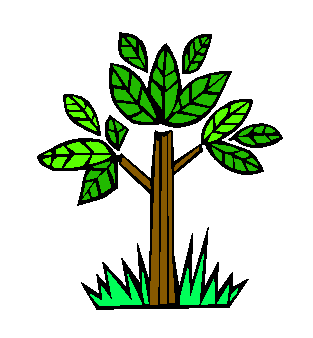
\includegraphics[width=5cm,clip]{ejem1.eps}
  \caption{Descripción.}
  \label{figura1}
\end{figure}


Este es un ejemplo de una referencia.

Podemos referirnos a un autor poniendo su cita directamente
\cite{Allen97}...

También podemos referirnos a un autor incluyendo su nombre en la
oración como ocurre con la propuesta de \namecite{allen2000}.

\section{Ejemplos de ejemplos y fórmulas}
En la fórmula \ref{formula1} se muestra...
\begin{equation}
\sum (a_n*b_n) \label{formula1}
\end{equation}

En el ejemplo \ref{ejemplo1} se muestra...
\begin{example}
Este es un ejemplo hecho utilizando el formato de los ejemplos.
\label{ejemplo1}
\end{example}

\section{Nueva sección}

El primer párrafo de la sección no lleva sangría. El resto del
texto vendrá con fuente Times New Roman tamaño 11 y justificado
por ambos lados.

Aquí tenemos distintos tipos de referencias según su publicación.

\begin{itemize}
\item Cita de un artículo en revista
\cite{Carletta96}.

\item Cita de un artículo en congreso
\cite{Connolly94}.

\item Cita de un libro \cite{Casares94}.

\item Cita de un informe técnico \cite{Ersan94}.
\end{itemize}

\section*{Agradecimientos}

Los siguientes párrafos llevan una sangría en la primera línea de
0,5 cm. El resto del texto vendrá con fuente Times New Roman
tamaño 11 y justificado por ambos lados.


\bibliographystyle{fullname_esp}
\bibliography{EjemploARTsepln}

\appendix
\section{Anexo 1: Descripción} Texto del anexo j klj ñlkj ñlkj ñlkj
lkj ñlkj lkj lkj lkj ñlkj ñlkj ñlkj ñlk jñlkj ñlkj ñlkj
ñlkjñlkjñlkjñlkjñlkjñlkj.

\section{Anexo 2: Descripción} Texto del anexo j klj ñlkj ñlkj ñlkj
lkj ñlkj lkj lkj lkj ñlkj ñlkj ñlkj ñlk jñlkj ñlkj ñlkj
ñlkjñlkjñlkjñlkjñlkjñlkj.

\end{document}
